\section{3D UNet}
\begin{figure}[ht!]
    \centering
    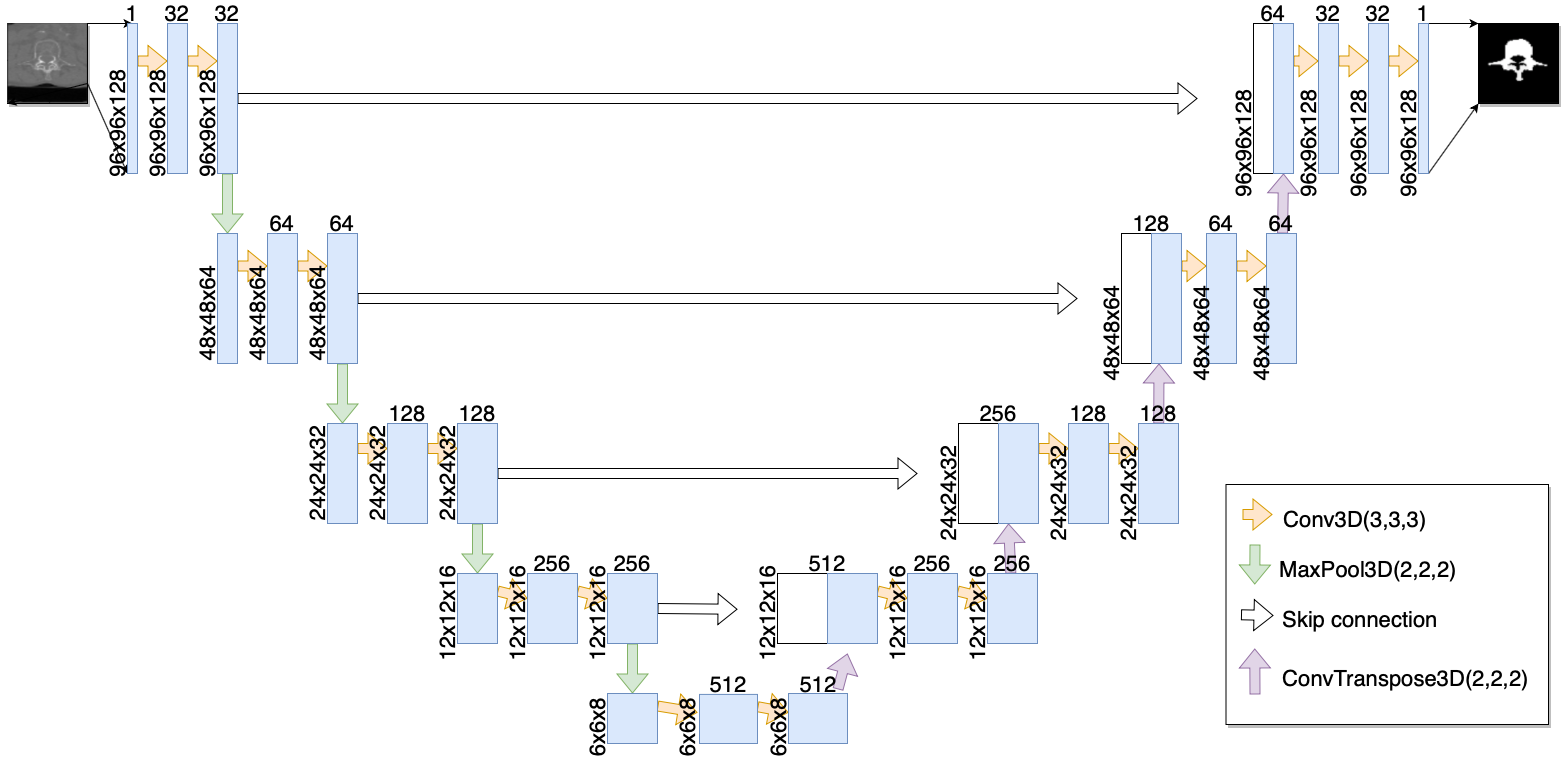
\includegraphics[width=1.\textwidth]{images/unet3d.png}
    \caption{3D UNet architecture}
    \label{fig:3D-unet}
\end{figure}

My architecture \ref{fig:3D-unet} is based on the original architecture of UNet \cite{unet2015} and Ultrasound Nerve Competition Tutorial \cite{jocic}. It is an encoder-decoder with skip connections between the same levels  of the contracting and the expansive path. The major difference is that my network accepts 3D images and also produces 3D outputs. Furthermore, all the operations: convolution, maxpooling and up-convolution are changed to work in the three-dimensional space. 3D filters used are: (3,3,3) for convolution, (2,2,2) for maxpooling and (2,2,2) for up-convolution. These filters ``slide'' through the image in all three dimensions, meaning they are capable of taking the third dimension into account and recognising features in the 3D context. Overview for the number of filters in each layer is in Table \ref{tab:neurons}.

Input to my network is of the size 96x96x128. There are 5 levels (Table \ref{tab:encoder-block}) in the architecture. Starting with the contracting path, the first level consists of 2 3Dconvolutions, 32 filters each, followed by ReLU. The output is then downsampled by 3Dmaxpooling, reducing its size by half. The number of convolutional filters doubles with each level, also doubling the number of 3D feature vectors. 

%up
The expanding path (Table \ref{tab:decoder-block}) starts by a 3Dup-convolution from the bottom level. This operation doubles the output resolution and also reduces the number of feature maps. These are then concantated with its counterpart feature maps from the contracting path. Then, again, 2 3Dconvolutions follow. The number of convolutional filters reduces by half on the way up. 

On the top of the expanding path, we are back to the original resolution of the input image. The very last convolutional layer depends on the task. For binary segmentation, the last layer consists of 1 (1,1,1) filter and sigmoid activation, outputting a volume of 96x96x128 with probabilities for whether the voxel belongs to the foreground class.

For multiclass segmentation, the last convolutional layer consists of 26 (1,1,1) filters (one for each class), with softmax as the activation function. The size of the output is 96x96x128x26, where probabilities for every voxel for belonging to each class a stored. 

%---------------------------------------------------------------

\begin{table}[]
\centering
\begin{tabular}{@{}ccc@{}}
\toprule
\multicolumn{1}{l}{Encoder layers} & \multicolumn{1}{l}{Decoder layers} & \multicolumn{1}{l}{Neurons} \\ \midrule
1, 2                               & 17, 18                             & 32                          \\
3, 4                               & 15, 16                             & 64                          \\
5, 6                               & 13, 14                             & 128                         \\
7, 8                               & 11, 12                             & 256                         \\
\multicolumn{2}{c}{9, 10}                                               & 512                         \\ \bottomrule
\end{tabular}
\caption[Number of neurons for each layer]{Number of neurons in 3D Convolutional layers. Layers 9 and 10 represent the bottom of the network. Numbering starts at with the first convolutional layer of the network and ends with the last layer before the output layer.}
\label{tab:neurons}
\end{table}

%---------------------------------------------------------------

\begin{table}[]
\centering
\begin{tabular}{@{}ccccc@{}}
\toprule
Layer          & Filter size & Strides & Padding & Activation \\ \midrule
3D Convolution & 3, 3, 3     & 1, 1, 1 & same    & ReLu       \\
3D Convolution & 3, 3, 3     & 1, 1, 1 & same    & ReLu       \\
3D MaxPooling  & 2, 2, 2     & 2, 2, 2 & same    &            \\ \bottomrule
\end{tabular}
\caption{Encoder block}
\label{tab:encoder-block}
\end{table}

%---------------------------------------------------------------

\begin{table}[]
\centering
\begin{tabular}{@{}ccccc@{}}
\toprule
Layer                     & Filter size & Strides & Padding & Activation \\ \midrule
3D Transposed Convolution & 2, 2, 2     & 2, 2, 2 & same    &            \\
3D Convolution            & 3, 3, 3     & 1, 1, 1 & same    & ReLu       \\
3D Convolution            & 3, 3, 3     & 1, 1, 1 & same    & ReLu       \\ \bottomrule
\end{tabular}
\caption{Decoder block}
\label{tab:decoder-block}
\end{table}




